\documentclass[a4paper,10pt]{article}
\usepackage[brazil]{babel}
\usepackage[utf8]{inputenc}
\usepackage{graphicx}
\begin{document}
\title{Relatório visualização de dados}
\author{Matheus Alves Diniz\\matheusad@dcc.ufmg.br \\
Breno Chaves Gabrich\\brenocg@dcc.ufmg.br}
\maketitle
\section{Introdução}
  As redes de computadores protagonizaram uma revolução nos meios de
  comunicação com a propagação da internet. Um host de uma rede de
  computadores tem várias camadas, como: hardware, enlace etc..

  Neste trabalho prático é contemplada e implementada a camada de enlace de
  uma rede, tendo esta várias etapas por si só , como por exemplo a checagem
  de erros, o enquadramento, entre outras que serão explicadas abaixo.

\section{Implementação}

  A implementação desse trabalho foi realizada na liguagem python,
  utilizando as interfaces de socket para estabelecer as conexões e a
  interface de struct para organizar os dados em binário em
  network byte order.

  É importante notar que todos os nós são full duplex, tanto enviando quanto
  recebendo mensagens, as explicações dadas abaixo
  se referem a como são feitas, nos dois modos, a recepção e envio de
  mensagens.

  Um resumo da implementação pode ser observado pelo diagrama da figura 1.

  \begin{figure}
  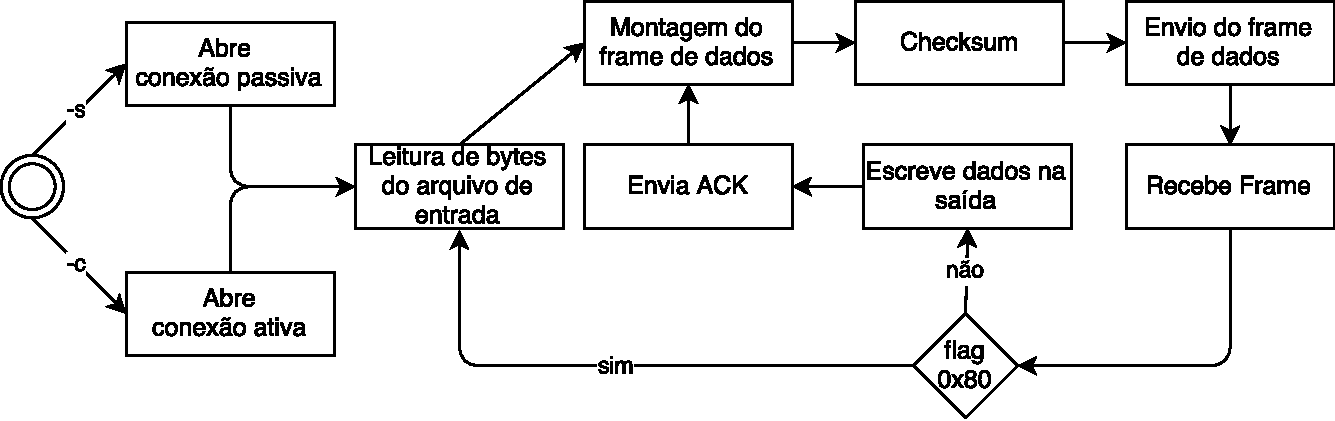
\includegraphics[scale=0.5]{diag.pdf}
    \caption{Diagrama de atividades do dccnet}
  \end{figure}

\subsection{Sincronização}
  Para sincronizar os quadros, recebe-se inicialmente 8 bytes. Esse 8 bytes
  são armazenados em um vetor e convertidos para string. Eles são então
  comparados com a string \"dcc023c2dcc023c2\". Caso a comparação seja
  negativa, o primeiro byte dessa string é descartado e um novo byte é
  recebido. A comparação é feita novamente, e o repete-se o procedimento de
  remover o byte mais antigo adicionar um novo byte até que a string de
  sincronização seja identificada corretamente.

\subsection{Checksum}
  O checksum faz a adição módulo 1 de todas as words de 16 bits do frame.
  O resultado do checksum é colocado no header do frame a ser enviado.
  A idéia é que o receptor deve fazer também essa soma e encontrar o mesmo
  resultado, caso contrário, algum dado veio corrompido.

  A entrada do checksum é uma string com a representação hexadecimal com
  preenchimento de zeros (e.g. 0x4 no campo length é representado pela string
  0004). Essa representação de entrada foi escolhida pois assim, cada word
  pode ser representada por 4 caractéres e então ser convertida para o inteiro
  correspondente.

\subsection{Receptor e Transmissor}
  Cada nó na rede funciona como transmissor e receptor, porém é necessário que
  um dos nós estabeleça a conexão passiva e o outro a conexão ativa. Assim,
  cada nó tanto envia frames (send) quanto recebe frames (recv). Porém,
  algum dos frames enviados e recebidos são de dados enquanto outros são
  de confirmação (ack).

  Para fazer essa distinção, utiliza-se a flag 0x80 que está presente no
  header de cada frame. Quando um frame recebido se trata de um ack de
  um dos frames enviados, o receptor enxerga uma flag 0x80, caso contrário,
  se trata de um frame de dados. O mesmo é válido na hora de se enviar um
  frame, naqueles de confirmação, o campo flag do header é marcado com a flag
  0x80.

\subsection{Camada de enlance}
  A camada de enlace tem várias etapas a se cumprir, de modo a garantir que
  o frame seja enviado corretamente, primeiro precisamos ler a entrada, a
  entrada é lida sempre de acordo com o tamanho do frame,
  e logo depois de ler, ela é convertida para string, para que possa ser
  utilizada em nossa implementação do checksum.

  Os frames foram especificados com um tamanho máximo de 256 bytes, qualquer
  mensagem maior que essa será quebrada em vários frames e enviada frame
  por frame, até que toda mensagem seja enviada. Essa decisão é importante
  para que caso algum frame se perda, não é necessário mandar novamente
  uma mensagem grande inteira, ao invés disso precisamos mandar apenas o
  parte perdida, que pode ser substancialmente menor que a mensagem.

  Como vários frames podem chegar para uma mensagem, é necessário um método
  para delimitar o final da mensagem. Para isso, utilizou-se a flag 0x40
  que marca o final da transmissão. Quando o receptor enxerga essa flag,
  ele sabe que nenhum frame a mais será transmitido, a não ser que o
  transmissor não consiga enxergar o ack deste último frame.

  Existe também um campo ID no header que permite identificar cada frame.
  Esse campo é necessário para que caso um frame seja enviado múltiplas vezes,
  o receptor consegue identificar que se trata de um mesmo frame e não escreve
  no arquivo de saída o dado duplicado.

\subsection{Envio de frames}
  O envio de frames é diferenciado para os frames de ack e os frames de dados.

  Os frames de confirmação simplesmente repassam os campos checksum e ID
  de um dos frames de dados recebidos. Nesse frame, é feita uma operação de 
  OR bit a bit com a flag e o imediato 0x80, marcando o frame como um frame
  de confirmação.

  Para o frame de dados, inicialmente o frame é montado como uma string para
  que possa ser calculado o seu checksum. Em seguida cada campo do header
  é convertido para binário com a função struct.pack e então enviado.
  Os dados também são são enviados, porém como a leitura já foi feita
  em binário, eles são enviados sem o pela transformação. Após o envio
  dos dados, o checksum calculado nesse etapa é salvo para que ele possa
  ser comparado no futuro com o frame de confirmação que será enviado pelo
  receptor.

\subsection{Recepção de frames}
  Ambos os frames de confirmação e de dados são recebidos da mesma maneira.

  Inicialmente é feita a sincronização até que se encontre a string
  \"dcc023c2dcc023c2\". Após encontrar essa string, o receptor então recebe
  2 bytes, correspondentes ao checksum, outros 2 bytes correspondentes ao
  campo length, 1 byte correspondente ao ID e outro byte correspondente à
  flag. Todos esses dados correspondem ao header do frame recebido.

  Todos esses bytes são convertidos para a representação em objetos de python
  através do struct.unpack. O servidor então recebe \textit{length} bytes,
  que correspondem aos dados do arquivo.

  O servidor então pega esse frame recebido e calcula o checksum.
  Caso o checksum calculado corresponda ao checksum recebido no header, o
  recebimento é avaliado como correto e um frame ACK é enviado ao transmissor.
  Caso contrário, o frame recebido é descartado.

\section{Testes}
  A corretude da transmissão foi avaliada através da comparação dos arquivos
  de saída de um nó com os arquivos de entrada do outro. Caso a transmissão
  tenha sido feita com sucesso, esses arquivos deveriam ser iguais, o que foi
  verificado através do programa diff.

  Alguns testes mais elaborados foram feitos com o intuito de se testar outras
  características da transmissão. Algumas mensagens de comprimento ímpar em
  bytes foram enviadas. Esse teste permite detectar que o checksum é capaz
  de anexar um byte 0x00 extra na mensagem para realizar o checksum mas
  esse byte não é transmitido, sendo descartado após o cálculo do checksum.

  Bytes aleatórios também foram enviados no meio do corpo do programa.
  Esse teste permite verificar que o receptor consegue corretamente
  identificar deslocamento de byte e então recuperar o alinhamento através
  dos bytes de sync no header.

  Arquivos com tamanho maior do que um frame também foram usados como entrada
  para que fosse verificado que múltiplos quadros são enviados corretamente
  e o quadro de fim de mensagem também é identificado de maneira certa.


\section{Conclusão}
  Podemos perceber com esse tp como é enviado um frame em uma conexão
  tcp por exemplo, é nítida a complexidade para se montar um frame com
  detecção de erros e sincronização.

  Temos a consciência que o frame gerado e enviado por esse trabalho, é muito
  parecido  com um frame enviado em uma situação real, as diferenças são
  na detecção erros, que geralmente é feita por um método mais robusto
  como o CRC, e no método de tratamento de erros, geralmente é usada uma
  janela deslizante, e não um stop and wait simples, apesar disso ainda assim
  foi possível exercitar conceitos aprendidos em sala e entendê-los melhor.

\end{document}
